\mysection{Pascal Triangle}

\begin{mysubsection}{}
    \begin{theorem}[thm:]{}
        \[{n-1\choose r}+{n-1\choose r+1}={n\choose r+1}.\]
    \end{theorem}

    \begin{proof}
        We may prove it with the pascal triangle. Or prove it directly by the combinatorics interpretations.
    \end{proof}

    Now, try to sum up each row of the pascal triangle. The sum of the first row, or row 0, equals 0. The sum of the second row, or row 1, equal 2. The sum of the third row, or row 2, equal 4. A few more iterations give us a conjecture that the sum of the n th row equals $2^n$, which leads us to the following theorem:

    \begin{theorem}[thm:]{}
        \[{n\choose 0}+{n\choose 1}+{n\choose 2}+\cdots +{n\choose n}=2^n.\]
    \end{theorem}

    \begin{proof}
        Since the sum of coefficients can be obtained by substituting $a=b=1$, hence the sum of each row is $2^n$. We may as well interpret as each entry equals the sum of the left entry and right entry on the previous row, which means the sum of row $n$ equals 2 times the sum of row $n-1$.

        The above sum is equal to the number of ways we can choose 1 object from $n$ objects plus 2 objects all the way up to choosing $n$ objects. Intuitively, this is all possible "choosings" for $n$ objects. Now, if we are to calculate the total possible "choosings" for $n$ objects, since each object can be either chosen or not chosen, this is equal to $\underbrace{2\times 2\times 2\times \cdots \times 2}_{\text{n times}}=2^n.$
    \end{proof}

    \begin{theorem}[thm:]{Hockey Stick Identity}
        \noindent\begin{minipage}{.65\linewidth}
        Start at any of the $1$ elements on the left or right side of Pascal's triangle. Sum elements diagonally in a straight line, and stop at any time. Then, the next element down diagonally in the opposite direction will equal that sum.
        If you start at the $r^{th}$ row and end on the $n^{th}$ row, this sum is
        \[\sum_{k=r}^{n}{k\choose r}={n+1\choose r+1}.\]
        \end{minipage}
        \begin{minipage}{.3\linewidth}
            
            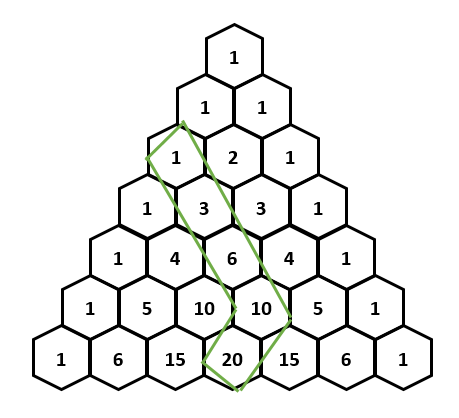
\includegraphics[width=\linewidth]{./co3_pic/PascalTriangleHockyStick.png}
        \end{minipage}
    \end{theorem}

    \begin{proof}
        We Since we have ${r\choose r}=1={r+1\choose r+1}$, we have 
        \[\sum_{k=r}^{n}{k\choose r}={r+1\choose r+1}+\sum_{k=r+1}^{n}{k\choose r}={r+2\choose r+1}+\sum_{k=r+2}^{n}{k\choose r}=\cdots ={n+1\choose r+1}.\]
    \end{proof}
\end{mysubsection}

